\documentclass{article}

\usepackage[utf8]{inputenc}
\usepackage{parskip}
\usepackage{enumitem}
\usepackage{graphicx}
\usepackage{float}
\usepackage{verbatim}
\usepackage{tabularx}
\usepackage{verbatim}
\usepackage{sectsty}
\usepackage{xcolor}
\usepackage{longtable}
\usepackage{array}
\usepackage{pdflscape}
\usepackage{hyperref}
\usepackage[table]{xcolor}
\graphicspath{ {../img/} }

\definecolor{sec-blue}{RGB}{77, 121, 255}
\definecolor{subsec-blue}{RGB}{153, 179, 255}
\sectionfont{\color{sec-blue}}
\subsectionfont{\color{subsec-blue}}

\title{DD}
\author{Leonardo Guglielmi, Francesco Lo Conte}
\date{\today\\Version 1}

\frenchspacing
\begin{document}
    \pagenumbering{arabic}
    
    \thispagestyle{empty} 
    \centering
    
    \includegraphics[width=8cm]{politecnico-di-milano-vector-logo.png}
    \vspace{1.5cm} 
    
    {\Large \textbf{COMPUTER SCIENCE AND ENGINEERING} \\}
    {\Large \textbf{SOFTWARE ENGINEERING II} \\}
    {\Large \textbf{2025 - 2026} \\} 
    
    \vspace{1.5cm}
    
    {\Huge \textbf{DD} \\}
    {\large Design Document \\}
    
    \vspace{0.5cm}
    {\Large \textit{Best Bike Paths}}
    
    \vspace{3cm} 

    {\Large \textbf{Authors:}} \\
    Leonardo Guglielmi, Francesco Lo Conte
    
    \vspace{0.5cm}
    {\Large \textbf{Version:}} \\
    1.0 \\
    (\today)
    
    \pagebreak
    \raggedright
    \tableofcontents
    \pagebreak

    \section{Introduction}

\subsection{Purpose}
The growing interest in cycling, whether as a recreational activity, a means of transportation, or a sport, brings with it a significant challenge: 
finding routes that are not only efficient, but also safe and well-maintained. Cyclists often lack reliable and up-to-date information on trail conditions, 
such as the presence of potholes, obstacles, or roads with little traffic. At the same time, many cyclists meticulously log their trips to monitor their performance, 
collecting valuable data that, however, remains siloed. This creates a gap where vital community knowledge about trail quality is not easily shared or accessible.
"Best Bike Paths" (BBP) aims to provide a solution. Commissioned by a cyclists' association, BBP will be a software system designed to create and manage a 
community-driven inventory of cycling routes. The platform will help bridge this information gap by allowing registered users to track their trips while 
simultaneously submitting detailed information on the condition of their routes. Other users, registered or not, will then be able to use this collective data 
to find and display the best possible cycling routes between two points, ranked by a quality score.

\subsubsection{Goals}
\begin{itemize}
    \item \textbf{G1:} A registered user wants to track their personal cycling activities and related performance statistics.
    \item \textbf{G2:} A registered user wants to contribute to the community inventory by sharing reliable information on the condition of the trails (e.g. quality, obstacles, potholes).
    \item \textbf{G3:} Any user (registered or not) wants to find and view the best cycling route between an origin and a destination, based on up-to-date and relevant data.
    \item \textbf{G4:} The cycling association aims to provide the community with a tool to create, consult, and maintain a reliable and centralized inventory of cycling routes.
\end{itemize}
\subsection{Scope}

The Best Bike Paths (BBP) system is designed to create, manage, and distribute a community-driven inventory of cycling paths, acting as a mediator 
between the physical conditions of the road network and the cyclists' need for safety. 
The scope of the application covers the entire lifecycle of path data: from its collection via mobile devices to its aggregation into a quality metric 
(Path Score) utilized for routing.

For this project, the following users interacting with the system have been identified:
\begin{itemize}
    \item \textbf{Registered User}
    \item \textbf{User}
\end{itemize}

A Registered User will be able to use the application to log and store their trips, tracking their cycling activities and related statistics. 
When available, this data can be enriched with weather information retrieved from external services. Furthermore, this user is the primary contributor to 
the inventory. They can enter route information in two ways:
\begin{enumerate}
    \item In \textbf{manual mode}, by actively specifying the route status (e.g., optimal, requires maintenance) and the presence of obstacles (e.g., potholes).
    \item In \textbf{automatic mode}, by allowing the app to acquire data from GPS and mobile device sensors while cycling, in order to automatically detect potential 
    problems such as potholes.
\end{enumerate}

For automatically collected data, the system will ask the user to confirm or correct the information before making it available to the community. 
Once confirmed or manually entered, this information becomes public.

Any user, whether registered or not, can benefit from the collected information. The user can specify a starting point and a destination. 
The system leverages third-party mapping services to identify valid physical routes and overlays them with BBP's inventory data. 
If a route is present in the inventory, it is displayed with its Path Score; otherwise, it is displayed without it.
If multiple routes exist, BBP will present them based on this score, calculated based on the route's status derived from
user-confirmed data.

\subsubsection{World phenomena}
%Eventi che accadono nel mondo reale, che il sistema non può né controllare né osservare. Sono le intenzioni o le azioni fisiche degli utenti.
\begin{itemize}
    \item \textbf{WP1:} The user fills up the registration form with its personal information.
    \item \textbf{WP2:} The user inserts an invalid email address in the registration form.
    \item \textbf{WP3:} The user inserts an email address in the registration form already used for another account.
    \item \textbf{WP4:} The registered user inserts the account credentials into the login form.
    \item \textbf{WP5:} The registered user inserts the wrong credentials into the login form.
    \item \textbf{WP6:} The registered user modifies an attribute.
    \item \textbf{WP7:} The registered user forgets the password.
    \item \textbf{WP8:} The registered user inserts the new password.
    \item \textbf{WP9:} The user searches for a path.
    \item \textbf{WP10:} The user inserts starting and destination points.
    \item \textbf{WP11:} The user stops cycling.
    \item \textbf{WP12:} The registered user evaluates a path.
    \item \textbf{WP13:} The registered user's personal device samples sensors data.
    \item \textbf{WP14:} The external weather service is unavailable.
    \item \textbf{WP15:} The external mapping system is unavailable.
    \item \textbf{WP16:} The registered user encounters a problem along a path.
    \item \textbf{WP17:} The registered user inserts a route problem information
    \item \textbf{WP18:} The registered user encounters a fixup problem.
    \item \textbf{WP19:} The registered user changes the problem status to "Resolved".
    \item \textbf{WP21:} The registered user confirms automatically detected problems.
    \item \textbf{WP22:} The registered user denies automatically detected problems
\end{itemize}

\subsubsection{Shared phenomena}
\paragraph{World controlled}
%Azioni che l'utente (mondo) compie sull'interfaccia del sistema. Il sistema deve reagirvi, ma non può avviarle. Sono gli input dell'utente.
\begin{itemize}
    \item \textbf{SP\_WC1:} The user registers themselves.
    \item \textbf{SP\_WC2:} The user submits to the system the registration form.
    \item \textbf{SP\_WC3:} The registered user sends the login form to the system.
    \item \textbf{SP\_WC4:} The registered user sends the attribute modification to the system.
    \item \textbf{SP\_WC5:} The registered user submits the new password.
    \item \textbf{SP\_WC6:} The registered user confirms to the system the account deletion.
    \item \textbf{SP\_WC7:} The user starts the search for a path in the app.
    \item \textbf{SP\_WC8:} The user submits to the system the starting and destination points.
    \item \textbf{SP\_WC9:} The user starts a ride.
    \item \textbf{SP\_WC10:} The external mapping service sends to the system a list of paths
    \item \textbf{SP\_WC11:} The user stops the ongoing ride.
    \item \textbf{SP\_WC12:} The user resumes the stopped ride.
    \item \textbf{SP\_WC13:} The user terminates the ride.
    \item \textbf{SP\_WC14:} The registered user submits the path evaluation.
    \item \textbf{SP\_WC15:} The registered user enables automatic data collection during an activity.
    \item \textbf{SP\_WC16:} The registered user's personal device sends to the system sampled data upon activity completion.
    \item \textbf{SP\_WC17:} The external weather service sends to the system weather conditions for a given path and datetime.
    \item \textbf{SP\_WC18:} The registered user submits a route problem information.
    \item \textbf{SP\_WC19:} The registered user reports the path fixup.
    \item \textbf{SP\_WC20:} The registered user submits detected problem confirmations.
    \item \textbf{SP\_WC21:} The registered user submits detected problems denials.
    \item \textbf{SP\_WC22:} The registered user sends to the user a request for its activity history.
    \item \textbf{SP\_WC23:} The registered user asks to the system to delete an activity.
\end{itemize}

\paragraph{Machine controlled}
%Azioni che il sistema (macchina) compie sull'interfaccia e che l'utente (mondo) può osservare. Sono gli output del sistema.
\begin{itemize}
    \item \textbf{SP\_MC1:} The system sends to the user the registration form.
    \item \textbf{SP\_MC2:} The system sends to the registered user the login form.
    \item \textbf{SP\_MC3:} The system asks to the registered user for which account it must reset the password
    \item \textbf{SP\_MC4:} The system asks to the user confirmation about account deletion.
    \item \textbf{SP\_MC5:} The system shows to the user a list of paths.
    \item \textbf{SP\_MC6:} The system asks to an external mapping service for a list of paths
    \item \textbf{SP\_MC7:} The system asks to the registered user to evaluate a path travelled during a completed activity.
    \item \textbf{SP\_MC8:} The system asks for weather conditions to an external weather service.
    \item \textbf{SP\_MC9:} The system shows to the registered user the activity summary with performances.
    \item \textbf{SP\_MC10:} The system shows to the registered user the activity summary with performances and weather conditions.
    \item \textbf{SP\_MC11:} The system asks confirmation to the registered user about detected problem during an activity.
    \item \textbf{SP\_MC12:} The system shows to the registered user its activity history.
\end{itemize}

\subsection{Definitions, Acronyms, Abbreviations}
    %questa sezione DEVE essere aggiornata durante la definizione del documento.
    This section contains the definitions for people that may not know what a specific concept is, acronyms and abbreviations used throughout the document.

    \subsubsection{Definitions}
    \begin{itemize}
        %dobbiamo inserire qualche altra definizione?
        \item \textbf{Bike Path:} a route deemed suitable for cycling. This includes paths with a proper bike track or roads where cars are rare and speed limits are 
        compatible with the average speed of a bike.
        \item \textbf{Ride:} a cycling trip made by a not-registered user.
        \item \textbf{Activity:} a personal record of a registered user's cycling trip, stored by the system to track performance metrics like distance and speed.
        \item \textbf{Publishable Information:} data about a bike path (e.g., status, obstacles) that a registered user has either entered
        making it available to the wider community.
        \item \textbf{Path Score:} a metric computed by BBP to rank route options. It is based on the status of the path and 
        its effectiveness in getting the user from their origin to their destination.   
        \item \textbf{Obstacle:} any significant element or condition on a cycle path that may represent a danger or hindrance to the cyclist (e.g. pothole).
    \end{itemize}

    \subsubsection{Acronyms}
    \begin{itemize}
        \item \textbf{BBP:} Best Bike Paths.           
        \item \textbf{GPS:} Global Positioning System.
        \item \textbf{API:} Application Programming Interface.
    \end{itemize}

    \subsubsection{Abbreviations}
    \begin{itemize}
        \item \textbf{G*:} Goal.
        \item \textbf{WP*:} World Phenomenon.
        \item \textbf{SP*:} Shared Phenomenon.
        \item \textbf{R*:} Requirement.
        \item \textbf{UC*:} Use Case.
        \item \textbf{D*:} Domain Assumption.
    \end{itemize}
    Note: asterisks are intended as a replacement for the number.
        
\subsection{Revision history}
    \begin{itemize}
        \item \textbf{Version 1.0 (23/12/2025)}
        \item \textbf{Vesrion 2.0 (10/01/2026)}: modified Use Case Diagram (Section 3.2.1), Sequence Diagrams 1,2,3,4,58,9,13 (Section 3.2.2) and Functional Requirement 
        RE7 (Section 3.2) after further definitions of those in the DD document.
    \end{itemize}

    \subsection{Reference documents}
    This document is based on the following materials:
    \begin{itemize}
        \item The specification of the RASD and DD assignment of the Software Engineering II course a.y. 2025/26.
        \item Course slides shared on WeBeep.
        \item Past Requirement Analysis and Specification Documents.
    \end{itemize}

\subsection{Document structure}
    \begin{enumerate}
        \item \textbf{Introduction:} a brief description of the project. It contains the main goals and objectives that the final system wants to achieve.
        \item \textbf{Overall description:} this section is a high-level representation of the system and of the interactions of the system with the other actors.
        \item \textbf{Specific requirements:} a detailed list of all the requirements needed for the system to achieve the goals. It contains valuable information for developers.
        \item \textbf{Formal analysis using Alloy:} a formal description of the model of the system with Alloy.
        \item \textbf{Effort spent:} the time spent on each section of the document, for each member of the group.
        \item \textbf{References:} reference to documents or tools used for writing this document.
    \end{enumerate}
    \pagebreak
    \section{Overall description}

\subsection{Overview}
The architecture is defined by two primary structural decisions: the adoption of a Microservices Architectural Style for 
the backend and a 4-Layer Architectural Approach to organize the logical and physical distribution of components.

\begin{figure}[H]
    \centering
    \makebox[\textwidth][c]{\includegraphics[width=1.1\textwidth]{DD/overview_diagram.pdf}}
    \label{fig:overview_diagram}
\end{figure}

For the BBP system we opted to base the architecture on a \textbf{4-Layer Approach}. This structural design was chosen to ensure 
a strict separation of concerns, thereby maximizing both maintainability and operational efficiency. The system is decomposed in 
the following distinct layers:
\begin{enumerate}
    \item \textit{Presentation Layer}, which serves as point of contact with the user. It is strictly responsible for 
    managing the User Interface (UI) and orchestrating the direct interaction flow with the user.

    \item \textit{Front-End Application Layer}, which encapsulates the logic of the mobile application. The features contained 
    in this layer  are those regarding the management of ongoing activities. Another key point of this layer is the execution 
    of an immediate, local analysis of raw data sampled during monitored activities, in order to reduce the volume of data transmission.

    \item \textit{Back-End Application Layer}, which acts as the central engine of the system. It houses the majority of the 
    system functionalities, implementing complex functionalities such as trip planning algorithms and comprehensive account management.

    \item \textit{Data Layer}, which functions are responsible for the secure storage and retrieval of system's data.

\end{enumerate}
Regarding the \textit{Back-End Application Layer}, the system adopts the \textbf{Microservices Architectural Style}. Rather than 
relying on a monolithic structure, this approach decomposes the system into a suite of small, autonomous services, with each service 
laser-focused on a specific bounded context within the domain.
Adopting this style provides a wide spectrum of strategic advantages. Primarily, it ensures high scalability and fault tolerance, while 
also allowing the architecture to leverage the benefits of geographical data distribution. Furthermore, it offers the flexibility to 
employ different programming technologies and languages best suited for specific services.
To align with this decentralized principle, the \textit{Data Tier} adopts a \textbf{distributed storage strategy}. Data is partitioned across 
different Database Management Systems (DBMS), where each instance is dedicated to a specific domain area—such as account management 
or trip handling, ensuring that the storage layer is as modular as the application logic it supports.
\pagebreak % 2.1
\subsection{Component View}

\begin{figure}[H]
    \centering
    \makebox[\textwidth][c]{\includegraphics[width=1.7\textwidth]{DD/component_diagram.pdf}}
    \caption{Component Diagram. In red are drown those components external our system; in blue those regarding 
    the Data tier, and in Green the mobile app residing on the user's device.}
    \label{fig:component_diagram}
\end{figure} % 2.2
\subsection{Deployment View}

\begin{figure}[H]
    \centering
    \makebox[\textwidth][c]{\includegraphics[width=1.7\textwidth]{DD/deployment_diagram.pdf}}
    \label{fig:deployment_diagram}
    \caption{Deployment Diagram. Allo these communications between deployed components are intended to be supervides by a circuit breaker.}
\end{figure}

\subsubsection*{User Device}
This refers to the mobile device used by the user, which serves as the host environment for the execution of the 
BBP mobile application.

\subsubsection*{Firewall}
Acting as the system's primary gatekeeper, this component monitors network data flow to detect anomalies and security threats. 
They are placed before the load balancers to secure inter-layer communications. The placement between the proxy services and
the external systems is made in order to protect the system from possible threatening message due to external interactions. 

\subsubsection*{Load Balancer}
Responsible for traffic distribution, these components serve as the entry point for requests destined for the API gateway layer. 
In order to facilitating the granular management of traffic on the specific requirements of each service macro-category, a dedicated l
oad balancing instance is utilized for each gateway type, 

\subsubsection*{Container \& API container}
Every system's service  is encapsulated in a container environment to enhance operational elasticity, allowing for the rapid instantiation of 
additional replicas as traffic volume increases.
 % 2.3
\subsection{Component Interfaces}

% ------------------------------
\subsubsection*{Account API Gateway}
\begin{table}[H]
    \centering
    \renewcommand{\arraystretch}{1.5}     
    \begin{tabular}{|l|p{0.8\textwidth}|}
        \hline
        Name & \multicolumn{1}{c|}{\textbf{Create account request}} \\ 
        \hline
        Signature & create\_acc\_req(name, surname, gender, birthdate, emailAddr, psw): void\\
        \hline
        Description & Forwards to the system the request of creating an account \\
        \hline
        Parameters &
            \begin{minipage}{0.8\textwidth}
            \smallskip
            \begin{itemize}
                \item  name: string, name of the user
                \item surname: string, surname of the user 
                \item gender: string, user gender
                \item birthdate: date, user birthdate
                \item email address (emailAddr): string, user email address 
                \item password(psw): string, account password 
            \end{itemize}
            \smallskip
            \end{minipage}  
        \\
        \hline
        Returned & \\
        \hline
         Exceptions & The submitted email it's already used, thereofore the account can't be created (already\_used\_error) \\
        \hline
    \end{tabular}
\end{table}

\begin{table}[H]
    \centering
    \renewcommand{\arraystretch}{1.5}     
    \begin{tabular}{|l|p{0.8\textwidth}|}
        \hline
        Name & \multicolumn{1}{c|}{\textbf{Send accont creation confimation}} \\ 
        \hline
        Signature & send\_create\_conf(regToken): bool \\
        \hline
        Description & Forwards to the system the confirmation to create an account\\
        \hline
        Parameters &  
            \begin{minipage}{0.8\textwidth}
            \smallskip
            \begin{itemize}
                \item registration token (regToken): string, token embedded into the confirmation link to validate the confirmation 
            \end{itemize}
            \smallskip
            \end{minipage} 
        \\
        \hline
        Returned & Returns an acknowledgemnt of account creation \\
        \hline
        Exceptions & The creation confirmation wasn't sent within 1 hour, therefore the request is expired (link\_expired\_error)\\
        \hline        
    \end{tabular}
\end{table}

\begin{table}[H]
    \centering
    \renewcommand{\arraystretch}{1.5}     
    \begin{tabular}{|l|p{0.8\textwidth}|}
        \hline
        Name & \multicolumn{1}{c|}{\textbf{Send login}} \\ 
        \hline
        Signature & sen\_login(emailAddr, psw): account\_info\\
        \hline
        Description & Forwards to the system the login request\\
        \hline
        Parameters &
            \begin{minipage}{0.8\textwidth}
            \smallskip
            \begin{itemize}        
                \item email address (emailAddr): string, user email address
                \item password (psw): string, account password
            \end{itemize}
            \smallskip
            \end{minipage} 
        \\
        \hline
        Returned & A map listing user attributes \\
        \hline
        Exceptions & \\
        \hline
    \end{tabular}
\end{table}

\begin{table}[H]
    \centering
    \renewcommand{\arraystretch}{1.5}     
    \begin{tabular}{|l|p{0.8\textwidth}|}
        \hline
        Name & \multicolumn{1}{c|}{\textbf{Modify attribute}} \\ 
        \hline
        Signature & modify\_attr(userId, attrId, newVal): bool \\
        \hline
        Description & Forwards to the system the request to modify the attribute specified with the new value\\
        \hline
        Parameters &
            \begin{minipage}{0.8\textwidth}
            \smallskip
            \begin{itemize}
                \item  userId: sting, unique identifier of the userId
                \item attrId: string, unique identifier of the attribute to be modified
                \item newVal: var, new value to assign to the attribute
            \end{itemize}
            \smallskip
            \end{minipage}    
        \\
        \hline
        Returned & Indicates that the update has been executed \\
        \hline
        Exceptions & \\
        \hline
    \end{tabular}
\end{table}

\begin{table}[H]
    \centering
    \renewcommand{\arraystretch}{1.5}     
    \begin{tabular}{|l|p{0.8\textwidth}|}
        \hline
        Name & \multicolumn{1}{c|}{\textbf{Password reset request}} \\ 
        \hline
        Signature & psw\_reset\_req(emailAddr): void \\
        \hline
        Description & Forwards to the system the request to chang password\\
        \hline
        Parameters &
            \begin{minipage}{0.8\textwidth}
            \smallskip
            \begin{itemize}
                \item  email address (emailAddr): string, user email address
            \end{itemize}
            \smallskip
            \end{minipage}    
        \\
        \hline
        Returned & \\
        \hline
        Exceptions & \\
        \hline
    \end{tabular}
\end{table}

\begin{table}[H]
    \centering
    \renewcommand{\arraystretch}{1.5}     
    \begin{tabular}{|l|p{0.8\textwidth}|}
        \hline
        Name & \multicolumn{1}{c|}{\textbf{Reset password cofirmation}} \\ 
        \hline
        Signature & reset\_psw\_conf(resetToken): reset\_psw\_form \\
        \hline
        Description & Forwards to the system the confirmation for the password reset\\
        \hline
        Parameters &
            \begin{minipage}{0.8\textwidth}
            \smallskip
            \begin{itemize}
                \item  reset token (resetToken): string, token embedded into the confirmation link to validate the password reset request
            \end{itemize}
            \smallskip
            \end{minipage}    
        \\
        \hline
        Returned & The reset password form with the token embedded \\
        \hline
        Exceptions & \\
        \hline
    \end{tabular}
\end{table}

\begin{table}[H]
    \centering
    \renewcommand{\arraystretch}{1.5}     
    \begin{tabular}{|l|p{0.8\textwidth}|}
        \hline
        Name & \multicolumn{1}{c|}{\textbf{Submit new password}} \\ 
        \hline
        Signature & submit\_new\_psw(newPsw, resetToken): bool\\
        \hline
        Description & Forwards to the system the new password given by the user \\
        \hline
        Parameters &
            \begin{minipage}{0.8\textwidth}
            \smallskip
            \begin{itemize}
                \item  new password (newPsw): string, new password chosen by the user
                \item reset token (resetToken): string, token embedded into the confirmation link to validate the password reset request
            \end{itemize}
            \smallskip
            \end{minipage}    
        \\
        \hline
        Returned & Indicates that the update has been executed  \\
        \hline
        Exceptions & \\
        \hline
    \end{tabular}
\end{table}

\begin{table}[H]
    \centering
    \renewcommand{\arraystretch}{1.5}     
    \begin{tabular}{|l|p{0.8\textwidth}|}
        \hline
        Name & \multicolumn{1}{c|}{\textbf{Send account deletion request}} \\ 
        \hline
        Signature & send\_delete\_acc(userId, emailAddr): void \\
        \hline
        Description & Forwards to the system the request to delete the account\\
        \hline
        Parameters &
            \begin{minipage}{0.8\textwidth}
            \smallskip
            \begin{itemize}
                \item  userId: sting, unique identifier of the userId
                \item email address (emailAddr): string, user email address
            \end{itemize}
            \smallskip
            \end{minipage}    
        \\
        \hline
        Returned & \\
        \hline
        Exceptions & \\
        \hline
    \end{tabular}
\end{table}

\begin{table}[H]
    \centering
    \renewcommand{\arraystretch}{1.5}     
    \begin{tabular}{|l|p{0.8\textwidth}|}
        \hline
        Name & \multicolumn{1}{c|}{\textbf{Confirm account deletion}} \\ 
        \hline
        Signature & acc\_del\_conf(delToken): bool\\
        \hline
        Description & Forwards to the system the account deletion confirmation\\
        \hline
        Parameters &
            \begin{minipage}{0.8\textwidth}
            \smallskip
            \begin{itemize}
                \item  deletion token (delToken): string, token embedded into the confirmation link to validate the account deletion request
            \end{itemize}
            \smallskip
            \end{minipage}    
        \\
        \hline
        Returned & Indicates that the deletion has been executed\\
        \hline
        Exceptions & \\
        \hline
    \end{tabular}
\end{table}
 % 2.4
\subsection{Runtime View}

\subsubsection*{[UC1] Account creation}
\begin{figure}[H]
    \centering
    \makebox[\textwidth][c]{
        \includegraphics[width=1.5\textwidth]{DD/sequence diagram/account_creation_sd_uc1.pdf}
    }
    \label{fig:sequence_diagram_1}
\end{figure} % 2.5
\subsection{Selected architectural styles and patterns}

\subsubsection*{Microservice architectural style}
The decision to adopt a Microservices architectural style was primarily driven by the inherent requirement for horizontal scalability. Unlike monolithic structures, this 
distributed approach focusses on splitting the whole system into small pieces, each one specialized on dealing with a specific task, allowing the system to scale specific 
components independently, enabling the infrastructure to adapt dynamically to fluctuating workloads in real-time. Furthermore, the fine-grained decomposition of services 
and the intelligent duplication of critical resources significantly enhance the system's overall resilience.

\subsubsection*{4-layer architecture}
To ensure a modular and scalable environment, we opted for a 4-tier architectural approach. This design allows us to separate system functionalities based on their logical domain while 
simultaneously defining how these components are distributed across physical hardware and network boundaries.
We have identified the following layers:
\begin{itemize} 
    \item \textbf{Presentation Layer}: This layer serves as the primary interface between the user and the system. It is responsible for rendering the UI components and facilitating user 
    interaction, allowing the user to interct easily with the system.

    \item \textbf{Front-end Application Layer}: This layer encapsulates the client-side business logic executed within the mobile application. It handles tasks like trip management, high-frequency 
    real-time data sampling and on-device pattern recognition for identifying issues during recorded trips. To handle the recognition task, we've chose to use pre-trained lightweight machine learning models.

    \item \textbf{Back-end Application Layer}: This layer comprises the core server-side logic and the various microservices offered by the platform. It is architected as a set of distributed server nodes, 
    where each service is decoupled to address specific functional domains, ensuring high availability and fault isolation.

    \item \textbf{Data Layer}: Dedicated to the persistence and orchestration of system information, this layer consists of a distributed database cluster. It manages data integrity and retrieval across the 
    different storage strategies based on the specific type of data is handling.
\end{itemize}

\subsubsection*{API Gateway}
To fortify system security and streamline the interaction between the client-side and server-side logic, we implemented the API Gateway pattern. By positioning the gateway as 
the sole entry point for all client requests, we effectively decouple the front-end from the internal microservices architecture. This abstraction layer enhances the system's 
security by encapsulating the internal service topology, thereby shielding the underlying services from direct external exposure. To mitigate the risk of a Single Point of Failure, 
the gateway is deployed across multiple instances, ensuring high availability and continuous service. Beyond acting as a reverse proxy, these gateways also perform the tasks of server-side 
load balancing and service discovery (see Section \ref{sec:other_design_decisions}).
Furthermore, we adopted for a differentiated gateway strategy by dividing the entry points into two specialized categories: the Account API Gateway and the Trip API Gateway. This granular 
approach allows each gateway to scale independently according to the specific needs of the underlying services (e.g. an exceptional number of trip requests won't affect the login service)

\subsubsection*{Proxy}
To prevent internal microservices from directly interfacing with external systems, we implemented a Proxy Service pattern. This pattern establishes a secure communication intermediary, 
creating a strictly controlled boundary between our internal infrastructure and third-party services. By routing all external traffic through these proxies, we implement a robust security 
perimeter where initial validation and security audits can be performed without exposing the internal services. Beyond security, this approach facilitates a more decoupled architecture. 
By abstracting the external service's specific API, our internal business logic remains indipendent from the third-party implementation.

\subsubsection*{Circuit breaker}
To prevent a single service slowing down other services, we placed some circuit breakers on those services which have to interact other services but that are not stricly related to their 
funcionning, like API Gatweays, or those connected with third-part system, for which we don't have garanteed reliability.
This kind of pattern allows the client service to monitor the called service in order to don't be slowd down by another service, avoiding a ripple effect that may cause to slow down a even
bigger portion of the system.

To safeguard the system against performance degradation caused by a restricted group of services, we implemented the Circuit Breaker pattern. This is particularly useful for services that interact 
with non-critical dependencies, such as the API Gateways, or services interfaced with third-party systems, where their reliability cannot be guaranteed.
By utilizing this pattern, the calling service actively monitors the health and response times of the invoked service. If a particular service begins to fail or exceeds predefined latency thresholds, 
the circuit "closes," immediately redirecting subsequent calls to a fallback mechanism. This fail-fast approach prevents the calling service from hanging indefinitely, thereby avoiding a ripple effect 
that could otherwise compromise the entire application's stability. % 2.6
\subsection{Other design decisions} \label{sec:other_design_decisions}

\subsubsection*{Server-side service discovery}
To enable the API Gateways to route traffic effectively, we integrated a Service Discovery mechanism on them. When a new service instance is initialized, it automatically registers itself. To ensure 
consistency across all nodes in the discovery service, this registration data is propagated throughout the entire discovery system using a Gossiping Protocol, ensuring all gateway nodes are updated eventually.
To maintain updated the services' status, each service instance transmits a periodic heartbeat to the discovery service. The API Gateways maintain a local cache of the service mapping. In the event that a 
gateway attempts to communicate with a service instance that has become unresponsive, the corresponding service-map cache record is invalidated.

\subsubsection*{Server-side load balancing}
To facilitate fluid system scalability and prevent performance bottlenecks, the API Gateway services integrate a server-side load balancing mechanism. This component acts as a traffic 
orchestrator, distributing incoming requests across multiple instances of a target microservice. By doing so, the gateway ensures that traffic is routed only to available nodes, preventing 
any single instance from becoming overwhelmed. This approach is helps to maintain high availability and consistent response times. 
By dynamically balancing the workload, the system can effectively absorb sudden spikes in traffic and maintain a seamless user experience.

\subsubsection*{Containers}
In order to take full advantage of the microservice architecture, we opted to deploy services with containers.
Deploying microservices with containers allow to encapsulate each service with it's own environment. This allows to easily scale the system based on the specific needs. This also grants a more reliable system due 
the fact that containerization ensures that a failure is contained within it, without causing problems to other instances of the same service.

\subsubsection*{Caches}
To enhance system availability, we implemented a robust caching layer for those services that could benefit from it. This strategy is particularly effective for services characterized by read-intensive workloads, like
those interfacing directly with the DBMSs. By serving requests from the cache, we significantly decrease response times.
Caching approch also allows the system to pre-compute results for some high-demand requests, avoiding to iterate complex and time-consuming operations on demand.

\subsubsection*{Differentiated Database}
To optimize the management of different data types, we adopted a diffretentiated data storage strategy, differentiating our database and data layer architecture into five distinct functional areas based on the type of
data is going to handle. This modular organization allows each domain to utilize the most efficient storage technology for the services that are going to use that data.
This division further enables a tailored approach to Data Consistency based on the criticality of the information:
\begin{itemize}
    \item \textbf{Strong Consistency}: For data where coherency among all nodes is non-negotiable (such as user credentials), the system can use Relational Database Management Systems.
    \item \textbf{Eventual Consistency}: For data types with less stringent consistency requirements, such as issue updates or path information, the system can rely on NoSQL technologies. By adopting an eventual consistency model, 
    the system can have higher availability. This trade-off allows the system to remain highly responsive and performant.
\end{itemize} % 2.7
    \pagebreak
    \section{User Interface Design}
    % Questo comando assicura che tutti i bottoni abbiano lo stesso stile (Grassetto + Corsivo)
    \newcommand{\uiElement}[1]{\textit{\textbf{#1}}}
    % ---------------------------------------------------------------------

    \subsection{Overview}
    The BBP user interface is designed according to "Minimal Attention UX" principles to ensure safety during mobile use.
    While the RASD defined the visual appearance through mockups, this section details the navigation logic and the structure of the transitions 
    between views, organized by functional areas.
    \pagebreak
    
    \subsection{Navigation Logic}

    \subsubsection{Entry Point and Authentication Flow}
    Access to the system is managed through the \textit{Login} screen, which acts as the main hub to direct the user towards the authenticated or 
    anonymous flow.

    \begin{figure}[H]
        \centering
        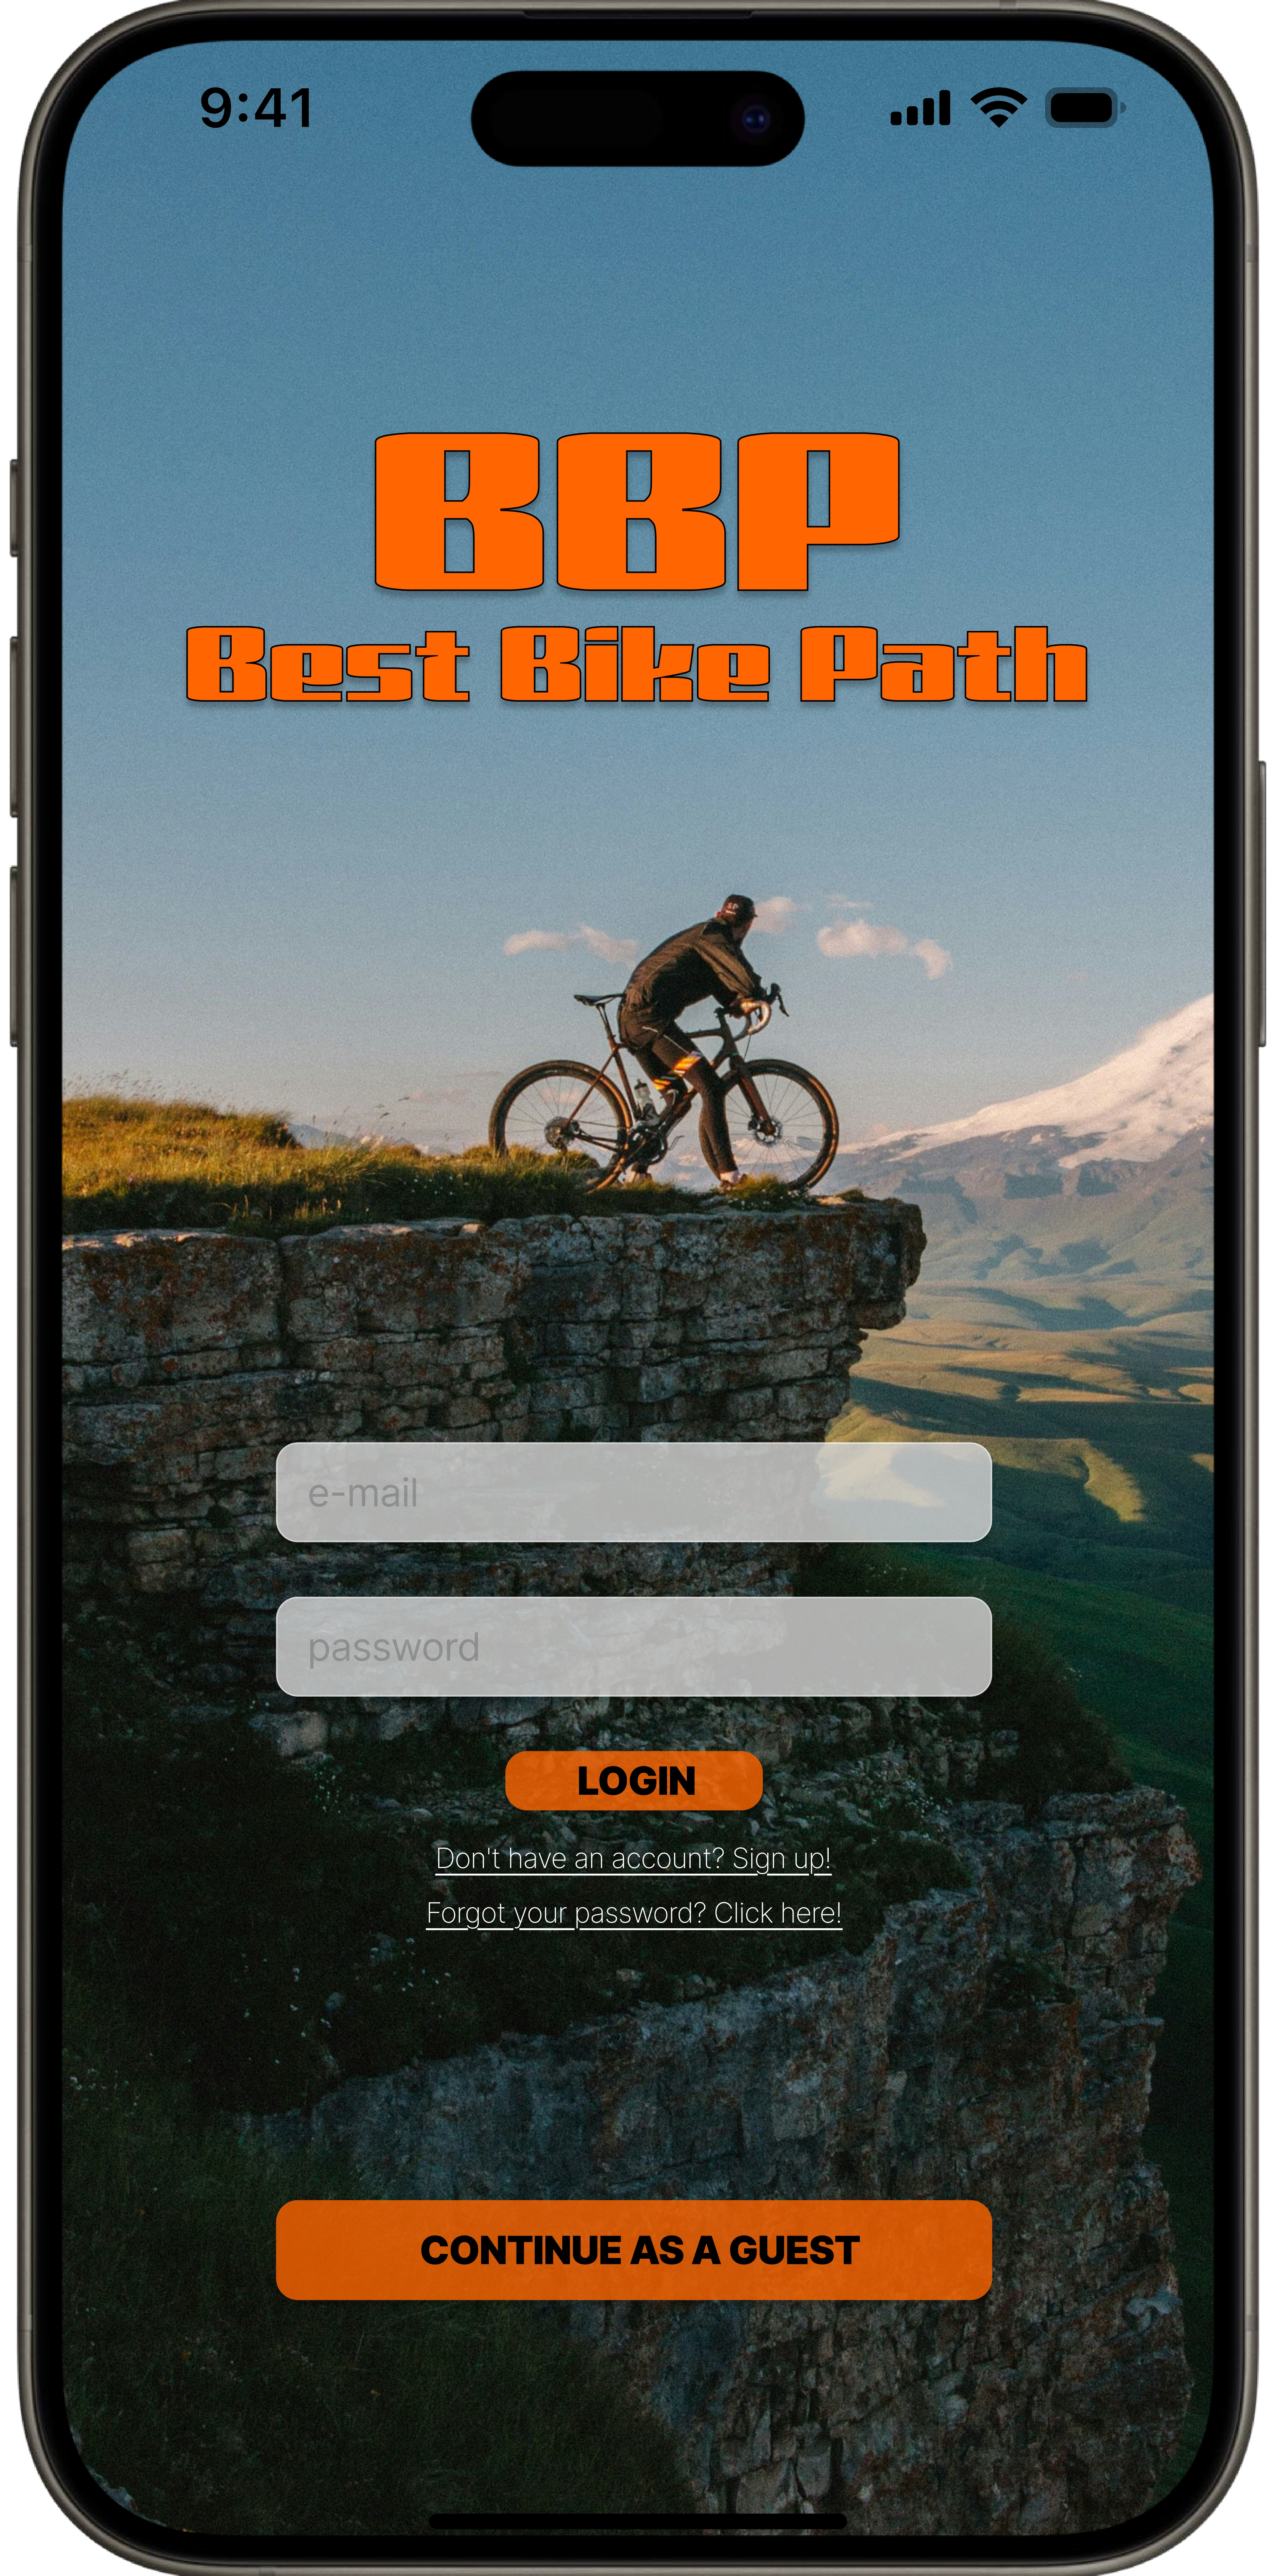
\includegraphics[width=0.5\textwidth]{RASD/mockups/mockup_login.jpg} 
        \caption{Start Screen and Access Logic}
        \label{fig:ui_login}
    \end{figure}

    \textbf{Transitions and Logic:}
    \begin{itemize}
        \item \textbf{Guest Path:} The \uiElement{Continue As A Guest} button instantiates an anonymous session and redirects the user directly to the 
        \textit{Map View} (see Fig. \ref{fig:ui_map}) with limited functionality.
        
        \item \textbf{Registered Path:} Entering credentials and tapping \uiElement{Login} validates the token; if successful, the user is redirected to the 
        \textit{Map View} with the Bottom Bar enabled.
        
        \item \textbf{Registration:} The \uiElement{Sign up} link opens the registration form, which, once completed, returns to this screen for the first login.
        
        \item \textbf{Password Recovery:} The \uiElement{Forgot your password?} link starts the external credential recovery flow via secure email. Once the 
        process is complete, the user remains on this screen to log in with the new password.
    \end{itemize}
    \pagebreak

    \subsubsection{Core Experience: Search and Tracking}
    The map is the central view of the application. From here, the user plans and takes action.

    \begin{figure}[H]
        \centering
        \includegraphics[width=0.5\textwidth]{RASD/mockups/mockup_search.jpg}
        \caption{Main Map View and Route Selection}
        \label{fig:ui_map}
    \end{figure}

    \textbf{Transitions and Logic:}
    \begin{itemize}
        \item \textbf{Route Selection:} Interacting with search results or tracks on the map updates the Bottom Sheet shown in the figure.
        
        \item \textbf{Start Navigation:} The \uiElement{Start} button initializes the Tracking state, placing the interface in "Driving Mode".
        
        \item \textbf{Alerts:} The \uiElement{List Alert} button opens a modal overlay listing known obstacles on the route.
        
        \item \textbf{Automatic Mode:} The \uiElement{Automatic mode} toggle switch allows the user to explicitly enable or disable sensor data acquisition for 
        the upcoming trip.
        
        \item \textbf{Sharing:} The \uiElement{Share} icon (top right) activates the operating system's native share sheet for sharing the route with other users.
        
        \item \textbf{Text View:} The \uiElement{List} icon (top left of the panel) switches the view from the graphical map to a text list of navigation directions.
    \end{itemize}
    \pagebreak
    
    \subsubsection{Data Governance Flow}
    At the end of a tracking session, the system prevents an immediate return to the Home page, forcing a critical data validation step.

    \begin{figure}[H]
        \centering
        \includegraphics[width=0.5\textwidth]{RASD/mockups/mockup_confirmation.jpg}
        \caption{Confirmation and Data Validation Screen}
        \label{fig:ui_confirm}
    \end{figure}

    \textbf{Transitions and Logic:}
    \begin{itemize}
        \item \textbf{Loop Closure:} This view is accessible only after the \texttt{Stop Recording} event and represents the mandatory Data Governance step.
        
        \item \textbf{Immediate Feedback:} The \uiElement{Trip Statistics} section immediately displays a summary of the performance metrics calculated
        for the trip just completed, such as distance, duration, average speed, etc.
        
        \item \textbf{Automatic Validation:} The \uiElement{Confirm} / \uiElement{Decline} toggles allow the user to validate or reject anomalies detected by the sensors, 
        preventing false positives.
        
        \item \textbf{Manual Enrichment:} The \uiElement{Do you want to add anything else?} button opens a context menu that allows the user to manually 
        report any issues not detected by the sensors or add specific details.
        
        \item \textbf{Qualitative Evaluation:} The \uiElement{Path Status} selector allows the user to assign an overall rating on the condition of the path 
        just completed (e.g., Optimal, Average, Poor).
        
        \item \textbf{Exit and Persistence:} The \uiElement{End Trip} button is the only way out: it finalizes the session, saves the confirmed data to the remote 
        database, and redirects the user to the \textit{History/Profile} view (Fig. \ref{fig:ui_history}).
    \end{itemize}
    \pagebreak

    \subsubsection{Persistence and History}
    The personal area allows asynchronous consultation of saved data.

    \begin{figure}[H]
        \centering
        \includegraphics[width=0.5\textwidth]{RASD/mockups/mockup_history.jpg}
        \caption{View Trip History}
        \label{fig:ui_history}
    \end{figure}

    \textbf{Transitions and Logic:}
    \begin{itemize}
        \item \textbf{Access:} Accessible via the \uiElement{Profile} tab in the Bottom Navigation Bar.
        \item \textbf{Detail:} Tapping on a card in the list opens the detail view of the individual trip.
    \end{itemize}
    \pagebreak
    \section{Requirements Traceability}

The following matrix maps each functional requirement to the system components responsible for its realization. An 'X' indicates that the component participates in satisfying the requirement.
\setlength\LTleft{-1.5cm}
{
\begin{longtable}{|c|p{3.0cm}|c|c|c|c|c|c|c|c|c|c|c|c|c|c|} 
    \hline
    \textbf{ID} & \textbf{Requirement} & 
    \rotatebox{90}{\textbf{Mobile App}} & 
    \rotatebox{90}{\textbf{Acc. API GW}} & 
    \rotatebox{90}{\textbf{Trip API GW}} & 
    \rotatebox{90}{\textbf{Acc. Creation Svc}} & 
    \rotatebox{90}{\textbf{Acc. Deletion Svc}} & 
    \rotatebox{90}{\textbf{Cred. Subsys.}} & 
    \rotatebox{90}{\textbf{Acc. Subsys.}} & 
    \rotatebox{90}{\textbf{Act. Handler Svc}} & 
    \rotatebox{90}{\textbf{Act. Storage Subsys.}} & 
    \rotatebox{90}{\textbf{Trip Planner Svc}} & 
    \rotatebox{90}{\textbf{Path Subsys.}} & 
    \rotatebox{90}{\textbf{Pub. Info Subsys.}} & 
    \rotatebox{90}{\textbf{Weather Proxx}} & 
    \rotatebox{90}{\textbf{Email Proxy}} \\
    \hline
    \endhead
    
    % --- AUTHENTICATION ---
    \textbf{R1} & Create an account & X & X & & X & & X & X & & & & & & & X \\ \hline
    \textbf{R2} & Log in & X & X & & & & X & X & & & & & & & \\ \hline
    \textbf{R3} & Reset password & X & X & & & & X & & & & & & & & X \\ \hline
    \textbf{R4} & Update profile info & X & X & & & & & X & & & & & & & \\ \hline
    \textbf{R5} & Delete account & X & X & & & X & X & & & & & & & & X \\ \hline
    
    % --- TRIP RECORDING ---
    \textbf{R6} & Start recording & X & & X & & & & & & & & X & & & \\ \hline
    \textbf{R7} & Pause/Resume & X & & & & & & & & & & & & &  \\ \hline
    \textbf{R8} & Track pos. \& stats & X & & & & & & & X & & & & & & \\ \hline
    \textbf{R9} & Retrieve weather & & & X & & & & & X & & & & & X & \\ \hline

    % --- DATA CONTRIBUTION ---
    \textbf{R10} & Report path status & X & & X & & & & & & & & & X & & \\ \hline
    \textbf{R11} & Submit feedback & X & & X & & & & & X & & & & X & & \\ \hline
    \textbf{R12} & Report problems & X & & X & & & & & & & & & X & & \\ \hline
    \textbf{R13} & Enable auto-detect & X & & & & & & & & & & & & & \\ \hline
    \textbf{R14} & Analyze anomalies & X & & & & & & & & & & & & & \\ \hline
    \textbf{R15} & Review anomalies & X & & & & & & & & & & & & & \\ \hline
    \textbf{R16} & Confirm anomaly & X & & X & & & & & X & & & & X & & \\ \hline

    % --- PATH PLANNING ---
    \textbf{R17} & Compute routes & X & & X & & & & & & & X & X & X & & \\ \hline
    \textbf{R18} & Visualize routes & X & & & & & & & & & X & X & & & \\ \hline
    \textbf{R19} & Path Score & & & & & & & & & & X & & X & & \\ \hline
    \textbf{R20} & Display obstacles & X & & X & & & & & & & & & X & & \\ \hline
    \textbf{R21} & Filter search & X & & X & & & & & & & X & X & & & \\ \hline

    % --- TRIP HISTORY ---
    \textbf{R22} & View list & X & & X & & & & & & X & & & & & \\ \hline
    \textbf{R23} & View trip details & X & & X & & & & & & X & & X & & & \\ \hline
    \textbf{R24} & Delete activity & X & & X & & & & & & X & & & & & \\ \hline
    \textbf{R25} & Search activity & X & & X & & & & & & X & & & & & \\ \hline
    \textbf{R26} & Filter history & X & & X & & & & & & X & & & & & \\ \hline
    
\end{longtable}
}
    \pagebreak
    \documentclass{article}
\usepackage[utf8]{inputenc}
\usepackage{parskip}
\usepackage{enumitem}
\usepackage{graphicx}
\usepackage{float}
\usepackage{verbatim}
\usepackage{tabularx}
\usepackage{verbatim}
\usepackage{sectsty}
\usepackage{xcolor}
\usepackage{longtable}
\usepackage{array}
\usepackage{pdflscape}
\usepackage{hyperref}
\usepackage[table]{xcolor}

\title{test_sec5_DD}
\author{Leonardo Guglielmi}
\date{January 2026}

\begin{document}
\section{Implementation, Integration and Test plan}

\subsection{Implementation Plan}
The system architecture allows for parallel development. However, adhering to the \textbf{Critical Component Strategy}, prioritizing high-risk and 
foundational modules ensures that the core value proposition is secured early in the lifecycle.

\subsection{Component Integration Analysis}
The following table classifies system components based on the \textbf{Impact of Failure}. The scale ranges from 1 to 5.

\definecolor{critical}{RGB}{255, 102, 102}   
\definecolor{high}{RGB}{255, 178, 102}      
\definecolor{medium}{RGB}{255, 255, 153}   
\definecolor{low}{RGB}{153, 255, 153}  

\begin{itemize}
    \item \textbf{\colorbox{critical}{4} - Critical:} Complete system outage or total loss of the application's core purpose.
    \item \textbf{\colorbox{high}{3} - High:} Major functionality unavailable, but the system may offer degraded service.
    \item \textbf{\colorbox{medium}{2} - Moderate:} Secondary features unavailable; core flow remains intact.
    \item \textbf{\colorbox{low}{1} - Low:} Auxiliary information missing or minor workflows blocked.
\end{itemize}  

\begin{table}[H]
    \centering
    \renewcommand{\arraystretch}{1.4}
    \footnotesize 
    \begin{tabular}{|l|p{4.5cm}|c|c|}
        \hline
        \textbf{Component} & \textbf{Rationale for Classification} & \textbf{Impact} \\
        \hline
        
        % LIVELLO 4 - CRITICO
        \textbf{Trip API Gateway} & 
        Single point of entry for all core features. If down, the App cannot communicate with the backend. & 
        \cellcolor{critical}\textbf{4} \\
        \hline
        
        \textbf{Path Subsystem} & 
        Provides map data and road network topology. Without it, no visualization or routing is possible. & 
        \cellcolor{critical}\textbf{4} \\
        \hline
        
        \textbf{Trip Planner Service} & 
        Core business logic. The primary goal of "Best Bike Paths" is finding routes. Without it, the app loses its purpose. & 
        \cellcolor{critical}\textbf{4} \\
        \hline
        
        % LIVELLO 3 - ALTO
        \textbf{Credentials Subsystem} & 
        Manages Authentication (Login) and Security. Critical for user access, though Guest Mode bypasses it. & 
        \cellcolor{high}\textbf{3} \\
        \hline
        
        \textbf{Account Subsystem} & 
        Essential for user persistence, but Guest Mode mitigates total failure. & 
        \cellcolor{high}\textbf{3} \\
        \hline
        
        \textbf{Activity Handler Service} & 
        Responsible for tracking rides. High value, but users could theoretically still use the map for visual navigation without active recording. & 
        \cellcolor{high}\textbf{3} \\
        \hline
        
        \textbf{Account API Gateway} & 
        Entry point for Auth/Profile operations. If down, login and registration fail, limiting the app to Guest features. & 
        \cellcolor{high}\textbf{3} \\
        \hline
        
        % LIVELLO 2 - MEDIO
        \textbf{Activity Storage Subsystem} & 
        Manages history. Failure prevents viewing past trips, but does not block new rides (which can be buffered locally). & 
        \cellcolor{medium}\textbf{2} \\
        \hline
        
        \textbf{Public Info Subsystem} & 
        Crowdsourcing logic (Issue Reporting, Scoring). Important for data enrichment, but the system functions without community reports. & 
        \cellcolor{medium}\textbf{2} \\
        \hline

        \textbf{Account Creation Service} & 
        Responsible to create new account. Important for overhall experience, but Guest Mode mitigates the inconvenience.&
        \cellcolor{medium}\textbf{2} \\
        \hline

        \textbf{Email Proxy Service} & 
        Used only for password reset or confirmation emails. Failure impacts a tiny fraction of daily user interactions, except for Account Creation. & 
        \cellcolor{medium}\textbf{2} \\
        \hline
    
        % LIVELLO 1 - BASSO
        \textbf{Weather Proxy Service} & 
        Auxiliary feature. Lack of weather data reduces UX quality but does not stop any core function. & 
        \cellcolor{low}\textbf{1} \\
        \hline

        \textbf{Account Deletion Service} & 
        Used for handle account elimination. The malfunctioning does not compromise the overall experience. & 
        \cellcolor{low}\textbf{1} \\
        \hline
        
    \end{tabular}
    \caption{Component Criticality}
    \label{tab:implementation_order}
\end{table}
\pagebreak

\subsection{Integration Strategy}
To balance the complexity of distributed microservices with the need for early risk mitigation, the project adopts a \textbf{Hybrid Integration Strategy}. 
This approach combines two distinct methodologies applied at different architectural levels:

\begin{enumerate}
    \item \textbf{Macro-Level: Risk-Driven Integration.} \\
    At the system level, components are integrated based on their criticality. 
    The "High Risk" subsystems are integrated first to verify the architectural viability of the solution.
    
    \item \textbf{Micro-Level: Bottom-Up Integration.} \\
    Within each specific subsystem, development follows a linear Bottom-Up path: 
    \textit{DBMS $\rightarrow$ Data Access Layer $\rightarrow$ Service Logic $\rightarrow$ API Interface}. 
    This ensures that each unit is stable before being exposed to the rest of the system.
\end{enumerate}

The integration sequence is dictated by the dependency graph below, structured to support this hybrid flow:

\begin{figure}[H]
    \centering
    \includegraphics[width=\textwidth]{DD/dependency_diagram.pdf}
    \caption{Dependency Graph highlighting the criticality of each module.}
    \label{fig:dep_graph}
\end{figure}

\mbox{} \\
The integration roadmap is divided into four phases:

\paragraph{Phase 1: The Critical Core} \mbox{} \\

The primary goal is to secure the application's core value: routing on a map.
\begin{itemize}
    \item \textbf{Action:} Parallel Bottom-Up construction of the \textit{Path Subsystem}, \textit{Trip Planner} and \textit{Trip API Gateway}.
    \item \textbf{Integration Point:} The \textit{Trip Planner} is connected to the \textit{Path Subsystem} and with the \textit{Trip API Gateway} . 
    \item \textbf{Validation:} Verification that the routing algorithm correctly returns a valid output, also by verifying the operations that pass by \textit{Trip Api Gateawy}.
\end{itemize}

\paragraph{Phase 2: Activity Section} \mbox{} \\

Once the core logic is validated, the modules related to activities and publishable info are developed. 
\begin{itemize}
    \item \textbf{Action:} Parallel development of \textit{Activity Storage Subsystem} and \textit{Public Info Subsystem}, follows the development of \textit{Activity Handler} .
    \item \textbf{Integration Point:} Connection of \textit{Activity Handler} to \textit{Activity Storage Subsystem} and \textit{Public Info Subsystem}. Then integrate \textit{Trip Planner} with \textit{Public Info Subsystem}.
    \item \textbf{Validation:} Confirmation that a registered user can simulate a ride and that the data is persisted. Verify that manual reports are correcty processed and stored. Verify the remaining funcionalities of \textit{Trip Planner} after the integration.
\end{itemize}

\paragraph{Phase 3: Account Section} \mbox{} \\

After main application functionalities are tested, core modules related to account management are developed.
\begin{itemize}
    \item \textbf{Action:} Develop simultaneously the \textit{Credential Subsystem} and \textit{ccount Subsystem}. After this, develop the secondary modules 
    \textit{Accoutn Creation} and \textit{Email Proxy}.
    \item \textbf{Integration Point:} Connect \textit{Email Proxy} and \textit{Account Creation} modules with their dependecies.
    \item \textbf{Validation:} Verify that all functionalities of the modules developed in this phase are working.
\end{itemize}


\paragraph{Phase 4: Gateway Aggregation} \mbox{} \\

The system is exposed to the outside world.
\begin{itemize}
    \item \textbf{Action:} Deployment of \textit{Trip API Gateway} and \textit{Account API Gateway}.
    \item \textbf{Integration Point:} Gateways are configured to route traffic to the services deployed in Phases 1 and 2.
    \item \textbf{Validation:} End-to-end API testing to verify authentication tokens and correct routing.
\end{itemize}

\paragraph{Phase 4: Auxiliary \& Client Integration} \mbox{} \\

Final polish and connection of external non-critical dependencies.
\begin{itemize}
    \item \textbf{Action:} Integration of \textit{Weather Proxy}, \textit{Account Deletion}, and the \textit{Mobile App}.
    \item \textbf{Integration Point:} The Mobile App connects to the live Gateways.
    \item \textbf{Validation:} User Acceptance Testing (UAT) and usability verification.
\end{itemize}
\mbox{} \\
\mbox{} \\
\subsection{Test Plan}
The testing strategy aligns with the hybrid integration approach, ensuring coverage from granular logic to system-wide workflows.

\subsubsection{Unit Testing}
Focuses on the correctness of the internal logic of each service, isolated from dependencies using mocks.
\begin{itemize}
    \item \textbf{Tools:} JUnit 5, Mockito.
    \item \textbf{Key Targets:} 
    \begin{itemize}
        \item \textit{Trip Planner:} Routing algorithm correctness on use-case graphs.
        \item \textit{Credentials:} Password hashing strength and JWT generation.
    \end{itemize}
\end{itemize}

\subsubsection{Integration Testing}
Verifies the interactions defined in the sequence diagrams.
\begin{itemize}
    \item \textbf{Tools:} REST Assured, TestContainers.
    \item \textbf{Key Targets:}
    \begin{itemize}
        \item \textit{Service-to-Service:} Ensure \textit{Activity Handler} correctly calls \textit{Weather Proxy} upon trip completion.
        \item \textit{Gateway-to-Service:} Verify that the API Gateway correctly handles service timeouts and load balancing.
    \end{itemize}
\end{itemize}

\subsubsection{System Testing}
Validates the fully integrated system against the functional requirements.
\begin{itemize}
    \item \textbf{Key Scenarios:}
    \begin{itemize}
        \item \textit{Full Ride Cycle:} Registration $\rightarrow$ Login $\rightarrow$ Search Route $\rightarrow$ Start Ride $\rightarrow$ Stop \& Save.
        \item \textit{Resilience:} Verify that the \textit{Guest Mode} remains functional even if the \textit{Account Subsystem} is forcefully taken offline (Simulated Failure).
    \end{itemize}
\end{itemize}

\subsubsection{Acceptance Testing}
Final validation performed by human users to assess UX and real-world performance.
\begin{itemize}
    \item \textbf{Focus:} Responsiveness of the map on mobile devices, GPS accuracy, and clarity of navigation instructions.
\end{itemize}

\end{document}

    \pagebreak

    \section{Effort Spent}
    \begin{table}[H]
        \centering
        \renewcommand{\arraystretch}{1.5}
        \begin{tabular}{|l|c|c|c|c|c|}
            \hline
            \textbf{Student} & \textbf{Section 1} & \textbf{Section 2} & \textbf{Section 3} & \textbf{Section 4} & \textbf{Section 5}\\
            \hline
            Guglielmi Leonardo & 1h & 39h & 1h & 2h &\\
            \hline
            Lo Conte Francesco & 5h & & 5h & 5h & 10h\\
            \hline
        \end{tabular}
        \caption{Effort spent by each team member per section}
        \label{tab:effort_spent}
    \end{table}
    \pagebreak
    
    \section{References}
    \begin{itemize}
        \item \textbf{Standards referenced in the document:}
        \begin{itemize}
            \item \textit{IEEE Std 1016-2009} - IEEE Standard for Information Technology—Systems Design—Software Design Descriptions.
            \item \textit{Regulation (EU) 2016/679} (GDPR) - General Data Protection Regulation.
            \item \textit{ISO/IEC 27001} - Information Security Management.
        \end{itemize}

        \item \textbf{Tools and Languages:}
        \begin{itemize}
            \item \textit{PlantUML} - Open-source tool used to generate Sequence Diagram via code.
            \item \textit{StarUML} - Software modeling tool used to create UML Diagram, with the exception of SDs.
            \item \textit{Draw.io} - Tool used to create Overview Diagram.
            \item \textit{Figma} - Tool used for User Interface (UI) mockups.
            \item \textit{Visual Studio Code} - Integrated Development Environment used for \LaTeX\ editing.
            \item \textit{Git \& GitHub} - Version control and collaborative platform.
            \item \textit{JUnit 5 \& Mockito} - Referenced frameworks for Unit Testing.
        \end{itemize}
    \end{itemize}
    \pagebreak

    % -------------------------------------------------------------
    \section{Declaration of GenAI Usage}
    The project was supported by the use of generative artificial intelligence tools during the development of this document. The use of these tools 
    was strictly limited to technical support, linguistic refinement, and syntax checking.

    \subsection*{Tools Used}
    \begin{itemize}
        \item \textbf{Model:} Google Gemini
        \item \textbf{Usage Scope:} Linguistic revision and technical typesetting support.
    \end{itemize}

    \subsection*{Description of Usage}
    The authors certify that they are the sole creators of the intellectual content, including all architectural decisions, design patterns selection, and 
    testing strategies. The usage of AI was limited to:

    \begin{itemize}
        \item \textbf{Linguistic Checking:} The tool was used to review the English grammar and vocabulary of the technical descriptions to ensure 
        clarity, professional tone, and correctness.
        \item \textbf{Technical Support for \LaTeX:} The tool provided assistance in troubleshooting compilation errors and formatting complex elements.
        \item \textbf{Design Choices Discussion:} The tool was used to discuss and challenge architectural decisions, helping the authors to evaluate 
        trade-offs and strengthen the rationale behind the final design.
        \item \textbf{Interface Description Automation:} The tool streamlined the development of Interface Description from Sequence Diagram by analyzing the PlantUML diagram code
        and generating the \LaTeX table, which was then refined through careful review by ourselfs.
        \end{itemize}

    \subsection*{Verification}
    All content processed for linguistic or technical review was manually verified by the authors to ensure it accurately reflects the original intent, 
    the architectural logic, and the project requirements defined in the RASD.


\end{document}